\documentclass{article}
\usepackage[T1]{fontenc}

\usepackage{graphicx}
\usepackage{listings}
\begin{document}

\title{FOSS Lab Report - Virtualisation}
\author{Gokul K\\[2\baselineskip]
Roll Number: 21\\[2\baselineskip]}
\date{8 March 2020}

\maketitle

\newpage

\tableofcontents

\newpage

\setcounter{section}{26}
\subsection{Aim}
Install and run a virtualisation environment (e.g., xen, kqemu, virtualbox or lguest)
to test applications, new kernels and isolate applications.

\newpage

\subsection{Installation}
To install virtualbox in Arch-derivative linux distro we need to run:
\begin{verbatim}
	sudo pacman -S virtualbox
\end{verbatim}
We may also need to manually load virtualbox modules by running:
\begin{verbatim}
	sudo modprobe vboxdrv
\end{verbatim}
In the case of any persisting errors, we may need to disable secure boot
and/or install kernel headers and virtualbox-dkms
\newline\newline\newline

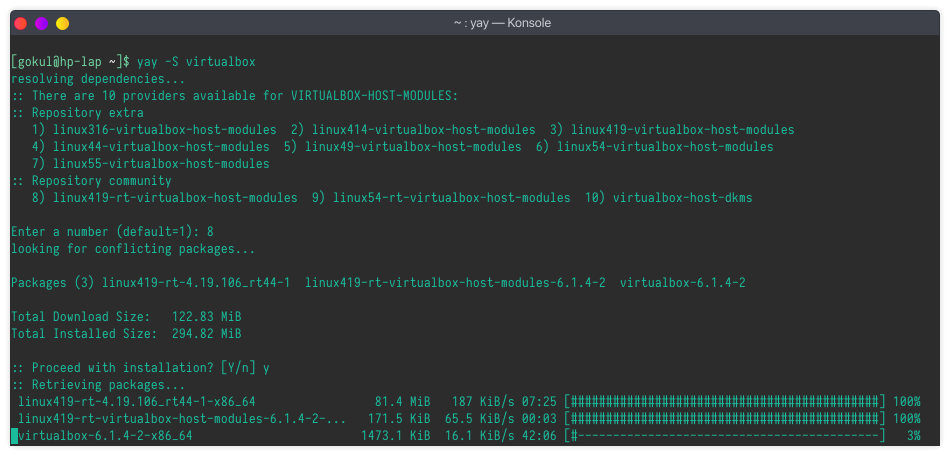
\includegraphics[width=1.2\textwidth]{img/p26/ss3.png}

\newpage

\subsection{Creating a VM}
Open virtualbox.
\newline\newline

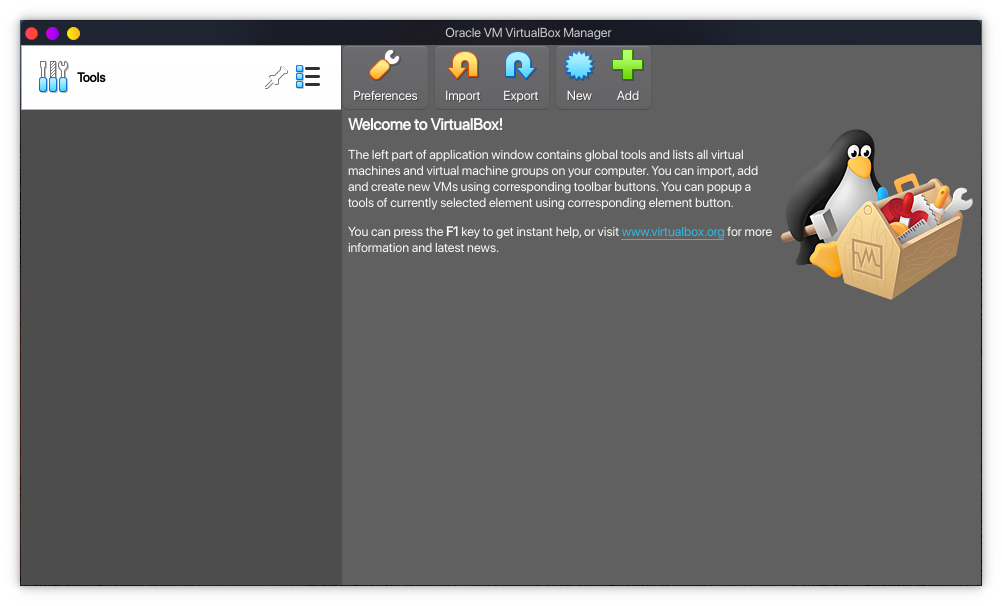
\includegraphics[width=1.2\textwidth]{img/p26/ss1.png}

Select New and follow the steps
\begin{itemize}
	\item Give a Name, VM location in the pop up. Select the OS type (Since we are installing
	Manjaro, we select Linux and Arch Linux (64 bit)) and click Next.
	\item Select the memory we need to allocate for the virtualbox in the next page. It is 
	recommended to select the optimum memory. Then click Next
	\item Select any of the option in the next page according to your preference
	\item If you selected to create a Virtual Disk then select how much hard disk space you
	need to allocate to the VM. Select a optimum value and click Create
\end{itemize}
Now the machine will be added to the Virtualbox
\newline\newline

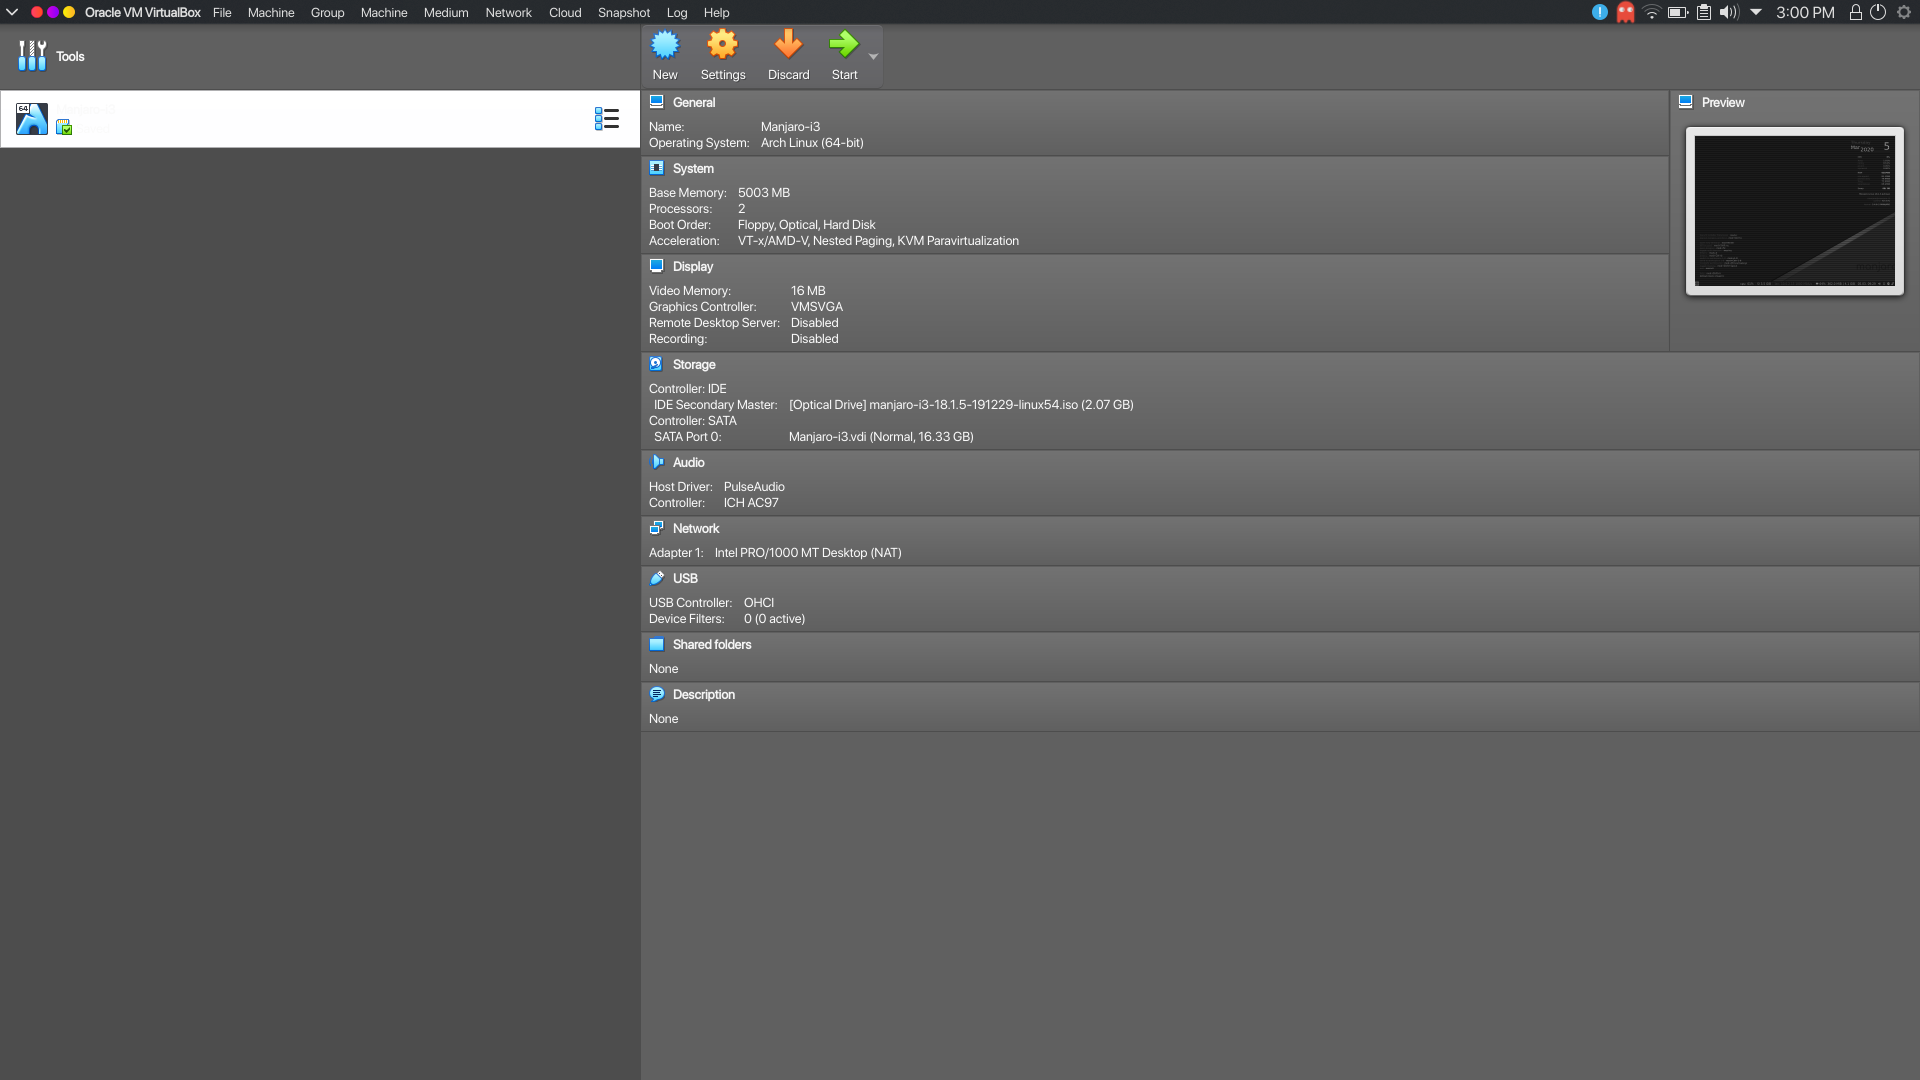
\includegraphics[width=1.2\textwidth]{img/p26/ss2.png}

\newpage

\subsection{Running the VM}
To run the VM we need to attach an install disk to the VM. To do so go to Settings, 
select Storage. Near the Controller: IDE select Add a Optical device
\newline
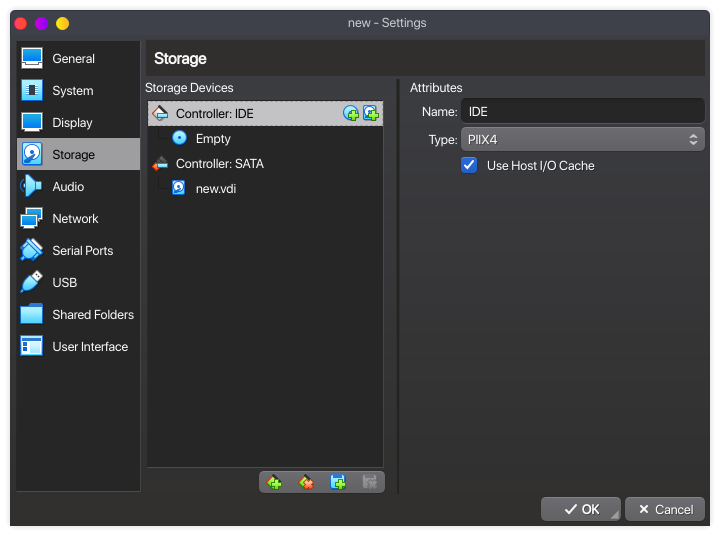
\includegraphics[width=1.2\textwidth]{img/p26/ss4.png}

In the new window, click Add and select the iso installation file
\newline
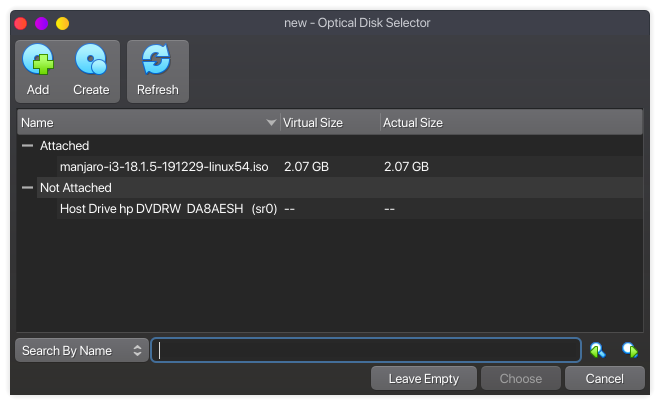
\includegraphics[width=1.2\textwidth]{img/p26/ss5.png}
Now select Choose.
Now run the VM by clicking Start. You will see the following window
\newline

\includegraphics[width=1.2\textwidth]{img/p26/ss6.png}

\newpage

\subsection{Output}
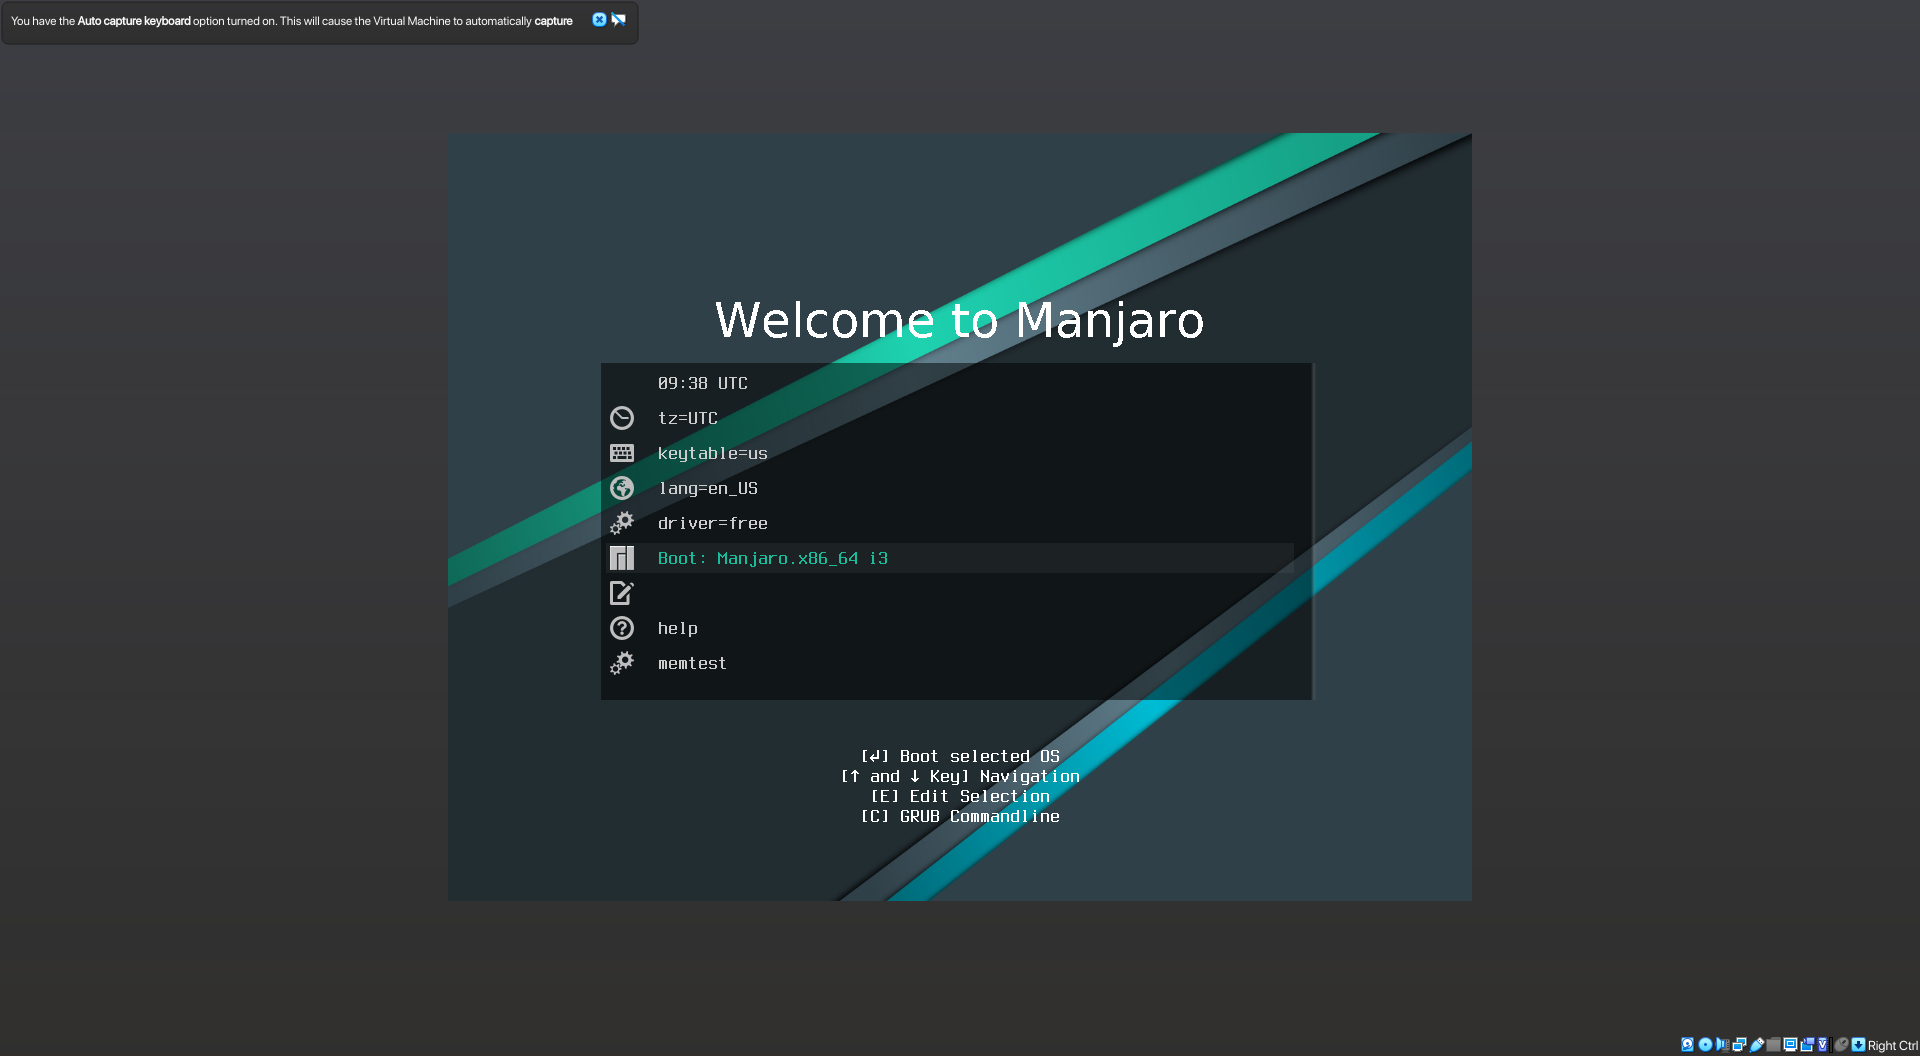
\includegraphics[width=1.2\textwidth]{img/p26/ss7.png}
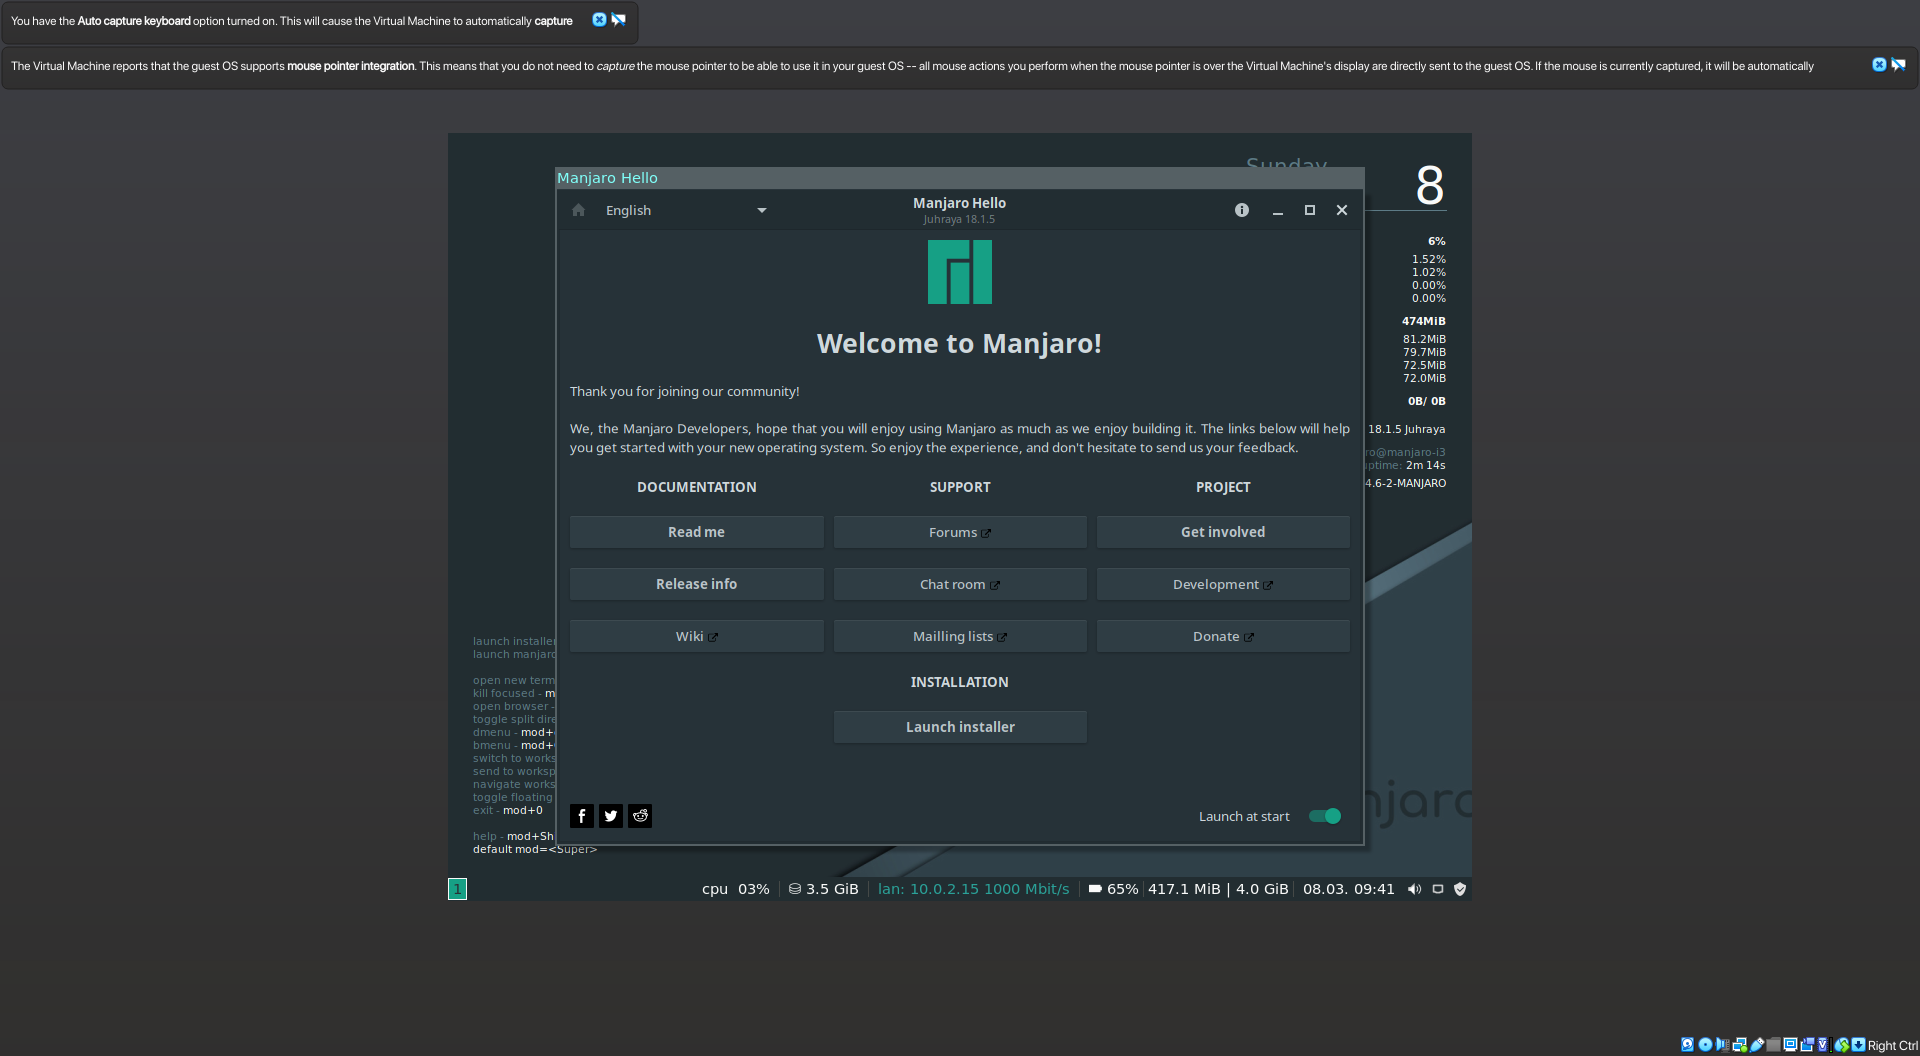
\includegraphics[width=1.2\textwidth]{img/p26/ss8.png}

\newpage

\subsection{Result}
Virtualbox is installed on Manjaro Linux (KDE Edition). A new VM is set up
and an iso of Manjaro Linux (i3 Edition) is attached to it. The VM is booted
and tested.
\end{document}